\documentclass[12pt,a4paper,portrait]{article}
%\setcounter{secnumdepth}{0}
\usepackage{gensymb}
\usepackage{pdflscape}
\usepackage{amsmath}
\usepackage{amssymb}
\usepackage{enumitem}
\usepackage{graphicx}
\usepackage{subcaption}
\usepackage{multirow}
\usepackage{sansmath}
\usepackage{pst-eucl}
\usepackage{multicol}
\usepackage{csquotes}
% Coding
\usepackage{listings}
\setlength{\parindent}{0pt}
\usepackage[obeyspaces]{url}
% Better inline directory listings
\usepackage{xcolor}
\definecolor{light-gray}{gray}{0.95}
\newcommand{\code}[1]{\colorbox{light-gray}{\texttt{#1}}}
\usepackage{adjustbox}
\usepackage[UKenglish]{isodate}
\usepackage[UKenglish]{babel}
\usepackage{float}
\usepackage[T1]{fontenc}
\usepackage{setspace}
\usepackage{sectsty}
\usepackage{longtable}
\newenvironment{tightcenter}{%
	\setlength\topsep{0pt}
	\setlength\parskip{0pt}
	\begin{center}
	}{%
	\end{center}
}
\captionsetup{width=\textwidth}
\usepackage{mbenotes} % to print table notes!
\usepackage{alphalph} % For extended counters!
% usage: \tabnotemark[3]\cmsp\tabnotemark[4]
\usepackage[colorlinks=true,linkcolor=blue,urlcolor=black,bookmarksopen=true]{hyperref}
\sectionfont{%			            % Change font of \section command
	\usefont{OT1}{phv}{b}{n}%		% bch-b-n: CharterBT-Bold font
	\sectionrule{0pt}{0pt}{-5pt}{3pt}}
\subsectionfont{
	\usefont{OT1}{phv}{b}{n}}
\newcommand{\MyName}[1]{ % Name
	\usefont{OT1}{phv}{b}{n} \begin{center}of {\LARGE  #1}\end{center}
	\par \normalsize \normalfont}
\makeatletter
\newcommand\FirstWord[1]{\@firstword#1 \@nil}%
\newcommand\@firstword{}%
\newcommand\@removecomma{}%
\def\@firstword#1 #2\@nil{\@removecomma#1,\@nil}%
\def\@removecomma#1,#2\@nil{#1}
\makeatother

\newcommand{\MyTitle}[1]{ % Name
	\Huge \usefont{OT1}{phv}{b}{n} \begin{center}#1\end{center}
	\par \normalsize \normalfont}
\newcommand{\NewPart}[1]{\section*{\uppercase{#1}}}
\newcommand{\NewSubPart}[1]{\subsection*{\hspace{0.2cm}#1}}
\renewcommand{\baselinestretch}{1.05}
\usepackage[margin=0.2cm]{geometry}
\date{}
\title{Pendulum on a cart on an inclined plane}
\author{Brenton Horne}

\begin{document}
	\maketitle
	\begin{figure}[H]
		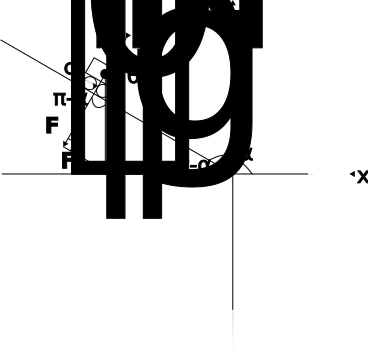
\includegraphics[width=300px]{Cart on an inclined plane with pendulum attached.png}
		\caption{Diagram of problem.}\label{fig1}
	\end{figure}
	
	Let the mass of the cart be $m_1$, the mass of the pendulum rod $m_{2r}$, and the mass of the pendulum bob $m_{2b}$.
	
	\tableofcontents
	
	\section{Coordinates and velocities}
	The $y$ coordinate of the cart's centre of mass is $y_{cart} = z\sin{\alpha} -c_0\cos{\alpha}$ where $c_0$ is the height of the cart's centre of mass relative to the inclined plane. As for its $x$ coordinate, it should be $x_{cart} = z\cos{\alpha}+c_0\sin{\alpha}$. Hence
	
	\begin{align*}
		\vec{r}_{cart} &= \begin{bmatrix}
			z\cos{\alpha} + c_0\sin{\alpha} \\
			z\sin{\alpha} - c_0\cos{\alpha}
		\end{bmatrix}.
	\end{align*}
	
	Let $c_1$ be the distance between the plane and the base of the pendulum. Then the coordinates of the base of the pendulum are
	
	\begin{align*}
		x_{base} &= z\cos{\alpha} + c_1\sin{\alpha} \\
		y_{base} &= z\sin{\alpha} - c_1\cos{\alpha}.
	\end{align*}
	
	As for the coordinates of rod's centre of mass it is
	
	\begin{align*}
		x_{rod} &= x_{base} - \dfrac{l\cos{(\theta+\alpha)}}{2}\\
		&= z\cos{\alpha} + c_1\sin{\alpha} - \dfrac{l\cos{(\theta+\alpha)}}{2} \\
		y_{rod} &= y_{base} - \dfrac{l\sin{(\theta+\alpha)}}{2}\\
		&= z\sin{\alpha} - c_1\cos{\alpha} - \dfrac{l\sin{(\theta+\alpha)}}{2}.
	\end{align*}
	
	Hence the time derivatives are:
	
	\begin{align*}
		\dot{x}_{rod} &= \dot{z}\cos{\alpha} + \dfrac{l\dot{\theta}\sin{(\theta+\alpha)}}{2} \\
		\dot{y}_{rod} &= \dot{z}\sin{\alpha} - \dfrac{l\dot{\theta}\cos{(\theta+\alpha)}}{2} \\
		v_{rod}^2 &= \dot{x}_{rod}^2 + \dot{y}_{rod}^2 \\
		&= \left(\dot{z}\cos{\alpha} + \dfrac{l\dot{\theta}\sin{(\theta+\alpha)}}{2}\right)^2 + \left(\dot{z}\sin{\alpha} - \dfrac{l\dot{\theta}\cos{(\theta +\alpha)}}{2}\right)^2 \\
		&= \dot{z}^2\cos^2{\alpha} + \dfrac{l^2 \dot{\theta}^2\sin^2{(\theta +\alpha)}}{4} + l\dot{z}\dot{\theta}\sin{(\theta+\alpha)}\cos{\alpha} + \dot{z}^2\sin^2{\alpha} - l\dot{z}\dot{\theta}\cos{(\theta +\alpha)}\sin{\alpha} + \dfrac{l^2\dot{\theta}^2\cos^2{(\theta+\alpha)}}{4}\\
		&= \dot{z}^2+\dfrac{l^2\dot{\theta}^2}{4}+l\dot{z}\dot{\theta}(\sin{(\theta+\alpha)}\cos{\alpha}-\cos{(\theta +\alpha)}\sin{\alpha})\\
		&= \dot{z}^2 + \dfrac{l^2\dot{\theta}^2}{4} + l\dot{z}\dot{\theta}\sin{\theta}.
	\end{align*}
	
	The coordinates of the bob centre of mass are
	
	\begin{align*}
		x_{bob} &= x_{base} - l\cos{(\theta+\alpha)}\\
		&= z\cos{\alpha} + c_1\sin{\alpha} - l\cos{(\theta+\alpha)}\\
		y_{bob} &= y_{base} - l\sin{(\theta+\alpha)}\\
		&= z\sin{\alpha} - c_1\cos{\alpha} - l\sin{(\theta+\alpha)}.
	\end{align*}
	
	Hence their time derivatives are
	\begin{align*}
		\dot{x}_{bob} &= \dot{z}\cos{\alpha} + l\dot{\theta}\sin{(\theta+\alpha)} \\
		\dot{y}_{bob} &= \dot{z}\sin{\alpha} - l\dot{\theta}\cos{(\theta+\alpha)} \\
		v_{bob}^2 &= \dot{x}_{bob}^2+\dot{y}_{bob}^2 \\
		&= (\dot{z}\cos{\alpha} + l\dot{\theta}\sin{(\theta+\alpha)})^2 + (\dot{z}\sin{\alpha} - l\dot{\theta}\cos{(\theta+\alpha)})^2 \\
		&= \dot{z}^2 \cos^2{\alpha} + l^2\dot{\theta}^2\sin^2{(\theta+\alpha)} + 2l\dot{z}\dot{\theta}\cos{\alpha}\sin{(\theta+\alpha)} + \dot{z}^2\sin^2{\alpha} + l^2\dot{\theta}^2\cos^2{(\theta+\alpha)} - 2l\dot{z}\dot{\theta}\sin{\alpha}\cos{(\theta+\alpha)} \\
		&= \dot{z}^2 + l^2\dot{\theta}^2 + 2l\dot{z}\dot{\theta}(\cos{\alpha}\sin{(\theta+\alpha)}-\sin{\alpha}\cos{(\theta+\alpha)}) \\
		&= \dot{z}^2 + l^2\dot{\theta}^2 +2l\dot{z}\dot{\theta}\sin{\theta}.
	\end{align*}
	
	The velocity squared of the bob is therefore $v_{bob}^2 = \dot{z}^2 + l^2 \dot{\theta}^2$.
	
	\section{Generalized basis vectors}
	\begin{align*}
		\dfrac{\partial \vec{r}_{cart}}{\partial z} &= \begin{bmatrix}
			\cos{\alpha} \\
			\sin{\alpha}
		\end{bmatrix} & \dfrac{\partial \vec{r}_{rod}}{\partial z} &= \begin{bmatrix}
		\cos{\alpha}\\
		\sin{\alpha}
		\end{bmatrix}\\
		\dfrac{\partial \vec{r}_{cart}}{\partial \theta} &= 0 & \dfrac{\partial \vec{r}_{rod}}{\partial \theta} &= \dfrac{l}{2}\begin{bmatrix}
			\sin{(\theta+\alpha)} \\
			-\cos{(\theta+\alpha)}
		\end{bmatrix}\\
		\dfrac{\partial \vec{r}_{bob}}{\partial z} &= \begin{bmatrix}
			\cos{\alpha} \\
			\sin{\alpha}
		\end{bmatrix} & \dfrac{\partial \vec{r}_{bob}}{\partial \theta} &= l\begin{bmatrix}
		\sin{(\theta+\alpha)} \\
		-\cos{(\theta+\alpha)}
		\end{bmatrix}.
	\end{align*}
	\section{Forces}
	Based on Figure \ref{fig1}, it is clear that $\vec{F}_g = -m_1g\hat{j}$.
	As for the forces acting on the cart, they are
	
	\begin{align*}
		\vec{F}_{\perp} &= m_1g\cos{(\pi-\alpha)}(-\sin{\alpha}, \cos{\alpha}) \\
		&= m_1g\cos{\alpha}(\sin{\alpha}, -\cos{\alpha})
	\end{align*}
	and
	
	\begin{align*}
		\vec{F}_{\parallel} &= -m_1g\sin{(\pi-\alpha)}(\cos{\alpha}, \sin{\alpha})\\
		&=- m_1g\sin{\alpha}(\cos{\alpha},\sin{\alpha}).
	\end{align*}
	
	Friction forces will be modelled as:
	
	\begin{align*}
		\vec{F}_{friction, cart} &= -(b_{cart}+c_{cart}v_{cart})\vec{v}_{cart} \\
		&= -(b_{cart} + c_{cart}\dot{z})\dot{z}\begin{bmatrix}
			\cos{\alpha} \\
			\sin{\alpha}
		\end{bmatrix} \\
		\vec{F}_{friction,rod} &= -(b_{rod}+c_{rod}v_{rod})\vec{v}_{rod} \\
		&= -\left(b_{rod} + c_{rod}\sqrt{\dot{z}^2+\dfrac{l^2\dot{\theta}^2}{4}+l\dot{z}\dot{\theta}\sin{\theta}}\right)\begin{bmatrix}
			\dot{z}\cos{\alpha} + \dfrac{l\dot{\theta}\sin{(\theta+\alpha)}}{2}\\
			\dot{z}\sin{\alpha} - \dfrac{l\dot{\theta}\cos{(\theta+\alpha)}}{2}
		\end{bmatrix}\\
		\vec{F}_{friction,bob} &= -(b_{bob}+c_{bob}v_{bob})\vec{v}_{bob} \\
		&= -\left(b_{bob} + c_{bob}\sqrt{\dot{z}^2+l^2\dot{\theta}^2+2l\dot{z}\dot{\theta}\sin{\theta}}\right)\begin{bmatrix}
			\dot{z}\cos{\alpha} + l\dot{\theta}\sin{(\theta+\alpha)}\\
			\dot{z}\sin{\alpha} - l\dot{\theta}\cos{(\theta+\alpha)}
		\end{bmatrix}.
	\end{align*}
	
	\section{Generalized forces}
	\begin{align*}
		Q_{z,cart} &= \vec{F}_{friction,cart} \cdot \dfrac{\partial \vec{r}_{cart}}{\partial z} \\
		&= -(b_{cart} + c_{cart}\dot{z})\dot{z}\begin{bmatrix}
			\cos{\alpha} \\
			\sin{\alpha}
		\end{bmatrix} \cdot \begin{bmatrix}
		\cos{\alpha} \\
		\sin{\alpha}
		\end{bmatrix} \\
		&= -(b_{cart} + c_{cart}\dot{z})\dot{z} \\
		Q_{z,rod} &= \vec{F}_{friction,rod} \cdot \dfrac{\partial \vec{r}_{rod}}{\partial z}\\
		&= -\left(b_{rod} + c_{rod}\sqrt{\dot{z}^2+\dfrac{l^2\dot{\theta}^2}{4}+l\dot{z}\dot{\theta}\sin{\theta}}\right)\begin{bmatrix}
			\dot{z}\cos{\alpha} + \dfrac{l\dot{\theta}\sin{(\theta+\alpha)}}{2}\\
			\dot{z}\sin{\alpha} - \dfrac{l\dot{\theta}\cos{(\theta+\alpha)}}{2}
		\end{bmatrix}\cdot \begin{bmatrix}
		\cos{\alpha}\\
		\sin{\alpha}
		\end{bmatrix} \\
		&= -\left(b_{rod} + c_{rod}\sqrt{\dot{z}^2+\dfrac{l^2\dot{\theta}^2}{4}+l\dot{z}\dot{\theta}\sin{\theta}}\right)\left(\dot{z}\cos^2{\alpha}+\dot{z}\sin^2{\alpha} + \dfrac{l\dot{\theta}\sin{(\theta+\alpha)}}{2}\cos{\alpha} - \dfrac{l\dot{\theta}\cos{(\theta+\alpha)}}{2}\sin{\alpha}\right) \\
		&= -\left(b_{rod} + c_{rod}\sqrt{\dot{z}^2+\dfrac{l^2\dot{\theta}^2}{4}+l\dot{z}\dot{\theta}\sin{\theta}}\right)\left(\dot{z}+\dfrac{l\dot{\theta}\sin{\theta}}{2}\right)\\
		Q_{z,bob} &= \vec{F}_{friction,bob} \cdot \dfrac{\partial \vec{r}_{bob}}{\partial z}\\
		&= -\left(b_{bob} + c_{bob}\sqrt{\dot{z}^2+l^2\dot{\theta}^2+2l\dot{z}\dot{\theta}\sin{\theta}}\right)\begin{bmatrix}
			\dot{z}\cos{\alpha} + l\dot{\theta}\sin{(\theta+\alpha)}\\
			\dot{z}\sin{\alpha} - l\dot{\theta}\cos{(\theta+\alpha)}
		\end{bmatrix} \cdot \begin{bmatrix}
		\cos{\alpha}\\
		\sin{\alpha}
		\end{bmatrix}\\
		&= -\left(b_{bob} + c_{bob}\sqrt{\dot{z}^2+l^2\dot{\theta}^2+2l\dot{z}\dot{\theta}\sin{\theta}}\right)\left(\dot{z}\cos^2{\alpha}+\dot{z}\sin^2{\alpha} + l\dot{\theta}\sin{(\theta+\alpha)}\cos{\alpha} - l\dot{\theta}\cos{(\theta+\alpha)}\sin{\alpha}\right)\\
		&= -\left(b_{bob} + c_{bob}\sqrt{\dot{z}^2+l^2\dot{\theta}^2+2l\dot{z}\dot{\theta}\sin{\theta}}\right)(\dot{z}+l\dot{\theta}\sin{\theta})\\
		Q_{z} &= -(b_{cart} + c_{cart}\dot{z})\dot{z} -\left(b_{rod} + c_{rod}\sqrt{\dot{z}^2+\dfrac{l^2\dot{\theta}^2}{4}+l\dot{z}\dot{\theta}\sin{\theta}}\right)\left(\dot{z}+\dfrac{l\dot{\theta}\sin{\theta}}{2}\right) \\
		&-\left(b_{bob} + c_{bob}\sqrt{\dot{z}^2+l^2\dot{\theta}^2+2l\dot{z}\dot{\theta}\sin{\theta}}\right)(\dot{z}+l\dot{\theta}\sin{\theta}).
	\end{align*}
	
	\begin{align*}
		Q_{\theta,cart} &= \vec{F}_{friction,cart} \cdot \dfrac{\partial \vec{r}_{cart}}{\partial \theta} \\
		&= 0\\
		Q_{\theta,rod} &= \vec{F}_{friction,rod} \cdot \dfrac{\partial \vec{r}_{rod}}{\partial \theta} \\
		&= -\left(b_{rod} + c_{rod}\sqrt{\dot{z}^2+\dfrac{l^2\dot{\theta}^2}{4}+l\dot{z}\dot{\theta}\sin{\theta}}\right)\begin{bmatrix}
			\dot{z}\cos{\alpha} + \dfrac{l\dot{\theta}\sin{(\theta+\alpha)}}{2}\\
			\dot{z}\sin{\alpha} - \dfrac{l\dot{\theta}\cos{(\theta+\alpha)}}{2}
		\end{bmatrix}\cdot\dfrac{l}{2}\begin{bmatrix}
		\sin{(\theta+\alpha)} \\
		-\cos{(\theta+\alpha)}
		\end{bmatrix} \\
		&= -\left(b_{rod} + c_{rod}\sqrt{\dot{z}^2+\dfrac{l^2\dot{\theta}^2}{4}+l\dot{z}\dot{\theta}\sin{\theta}}\right)\dfrac{l}{2}\left(\dot{z}\cos{\alpha}\sin{(\theta+\alpha)}+\dfrac{l\dot{\theta}\sin^2{(\theta+\alpha)}}{2} - \dot{z}\sin{\alpha}\cos{(\theta+\alpha)} \right.\\
		&\left.+ \dfrac{l\dot{\theta}\cos^2{(\theta+\alpha)}}{2}\right) \\
		&= -\left(b_{rod} + c_{rod}\sqrt{\dot{z}^2+\dfrac{l^2\dot{\theta}^2}{4}+l\dot{z}\dot{\theta}\sin{\theta}}\right)\dfrac{l}{2}\left(\dot{z}\sin{\theta}+\dfrac{l\dot{\theta}}{2}\right)\\
		Q_{\theta,bob} &= \vec{F}_{friction,bob} \cdot \dfrac{\partial \vec{r}_{bob}}{\partial \theta} \\
		&= -\left(b_{bob} + c_{bob}\sqrt{\dot{z}^2+l^2\dot{\theta}^2+2l\dot{z}\dot{\theta}\sin{\theta}}\right)\begin{bmatrix}
			\dot{z}\cos{\alpha} + l\dot{\theta}\sin{(\theta+\alpha)}\\
			\dot{z}\sin{\alpha} - l\dot{\theta}\cos{(\theta+\alpha)}
		\end{bmatrix} \cdot l\begin{bmatrix}
		\sin{(\theta+\alpha)} \\
		-\cos{(\theta+\alpha)}
		\end{bmatrix}\\
		&= -\left(b_{bob} + c_{bob}\sqrt{\dot{z}^2+l^2\dot{\theta}^2+2l\dot{z}\dot{\theta}\sin{\theta}}\right)l\left(\dot{z}\cos{\alpha}\sin{(\theta+\alpha)} + l\dot{\theta}\sin^2{(\theta+\alpha)}-\dot{z}\sin{\alpha}\cos{(\theta+\alpha)}\right. \\
		&\left.+ l\dot{\theta}\cos^2{(\theta+\alpha)}\right)\\
		&= -\left(b_{bob} + c_{bob}\sqrt{\dot{z}^2+l^2\dot{\theta}^2+2l\dot{z}\dot{\theta}\sin{\theta}}\right)l(\dot{z}\sin{\theta}+l\dot{\theta})\\
		Q_{\theta} &= -\left(b_{rod} + c_{rod}\sqrt{\dot{z}^2+\dfrac{l^2\dot{\theta}^2}{4}+l\dot{z}\dot{\theta}\sin{\theta}}\right)\dfrac{l}{2}\left(\dot{z}\sin{\theta}+\dfrac{l\dot{\theta}}{2}\right) \\
		&-\left(b_{bob} + c_{bob}\sqrt{\dot{z}^2+l^2\dot{\theta}^2+2l\dot{z}\dot{\theta}\sin{\theta}}\right)l(\dot{z}\sin{\theta}+l\dot{\theta})
	\end{align*}
	
	\section{Potential energy}
	Hence the potential energy of the cart under gravity is: 
	
	\begin{align*}
		V_{cart} &=-\int \vec{F}_{\parallel} \cdot d\vec{r} \\
		&= -\int_z^0 m_1g\sin{\alpha}(\cos{\alpha}, \sin{\alpha}) \cdot -(\cos{\alpha}, \sin{\alpha}) dz \\
		&= m_1gz\sin{\alpha}
	\end{align*}
	
	As for the pendulum, its potential energy is:
	
	\begin{align*}
		V_{pendulum} &= m_{2r} gy_{rod} + m_{2b}gy_{bob} \\
		&= m_{2r}g\left(z\sin{\alpha} - c_1\cos{\alpha} - \dfrac{l\sin{(\theta+\alpha)}}{2}\right) + m_{2b}g\left(z\sin{\alpha} - c_1\cos{\alpha} -l\sin{(\theta+\alpha)}\right)
	\end{align*}
	
	The $c_1$ terms are constants, so dropping them:
	
	\begin{align*}
		V_{pendulum} &= m_{2r}g\left(z\sin{\alpha} - \dfrac{l\sin{(\theta+\alpha)}}{2}\right) + m_{2b}g\left(z\sin{\alpha} - l\sin{(\theta+\alpha)}\right).
	\end{align*}
	
	Hence the potential energy is
	
	\begin{align*}
		V &= V_{cart} + V_{pendulum} \\
		&= m_1gz\sin{\alpha} + m_{2r}g\left(z\sin{\alpha}- \dfrac{l\sin{(\theta+\alpha)}}{2}\right) + m_{2b}g\left(z\sin{\alpha} - l\sin{(\theta+\alpha)}\right) \\
		&= (m_1+m_{2r}+m_{2b})gz\sin{\alpha} -\left(\dfrac{m_{2r}}{2}+m_{2b}\right)gl\sin{(\theta+\alpha)}.
	\end{align*}
	
	\section{Kinetic energy}
	The kinetic energy of the system is therefore
	
	\begin{align*}
		T &= T_{cart} + T_{rod} + T_{bob} \\
		&= \dfrac{m_1}{2} \dot{z}^2 + \dfrac{m_{2r}}{2}\left(\dot{z}^2+\dfrac{l^2\dot{\theta}^2}{4}+l\dot{z}\dot{\theta}\sin{\theta}\right)+\dfrac{m_{2r}}{24}l^2\dot{\theta}^2 + \dfrac{m_{2b}}{2}(\dot{z}^2+l^2\dot{\theta}^2+2l\dot{z}\dot{\theta}\sin{\theta})\\
		&= \dfrac{m_1+m_{2r}+m_{2b}}{2}\dot{z}^2 + \dfrac{l^2\dot{\theta}^2}{6}(m_{2r}+3m_{2b}) + \dfrac{l\dot{z}\dot{\theta}\sin{\theta}}{2}(m_{2r}+2m_{2b}).
	\end{align*}
	
	\section{Lagrangian}
	\begin{align*}
		\mathcal{L} &= T - V\\
		&= \dfrac{m_1+m_{2r}+m_{2b}}{2}\dot{z}^2 + \dfrac{l^2\dot{\theta}^2}{6}(m_{2r}+3m_{2b}) + \dfrac{l\dot{z}\dot{\theta}\sin{\theta}}{2}(m_{2r}+2m_{2b}) - (m_1+m_{2r}+m_{2b})gz\sin{\alpha}\\ &+\dfrac{gl\sin{(\theta+\alpha)}}{2}(m_{2r}+2m_{2b})\\
		&= \dfrac{m_1+m_{2r}+m_{2b}}{2}(\dot{z}^2 - 2gz\sin{\alpha})+\dfrac{l^2\dot{\theta}^2}{6}(m_{2r}+3m_{2b}) + \dfrac{m_{2r}+2m_{2b}}{2}\left(l\dot{z}\dot{\theta}\sin{\theta}+gl\sin{(\theta+\alpha)}\right)
	\end{align*}
	
	\section{Euler-Lagrange equations}
	\begin{align*}
		p_{z} &= \dfrac{\partial \mathcal{L}}{\partial \dot{z}} \\
		&= (m_1+m_{2r}+m_{2b})\dot{z} + \dfrac{m_{2r}+2m_{2b}}{2}l\dot{\theta}\sin{\theta} \\
		\dot{p}_{z} &= (m_1+m_{2r}+m_{2b})\ddot{z} + \dfrac{m_{2r}+2m_{2b}}{2}l\left(\ddot{\theta}\sin{\theta} + \dot{\theta}^2\cos{\theta}\right) \\
		F_{z} &= \dfrac{\partial \mathcal{L}}{\partial z} \\
		&= -g\sin{\alpha}(m_1+m_{2r}+m_{2b}) \\
		\dot{p}_{z} - F_z &= (m_1+m_{2r}+m_{2b})\ddot{z} + \dfrac{m_{2r}+2m_{2b}}{2}l\left(\ddot{\theta}\sin{\theta} + \dot{\theta}^2\cos{\theta}\right) +g\sin{\alpha}(m_1+m_{2r}+m_{2b}) \\
		&= (m_1+m_{2r}+m_{2b})(\ddot{z} + g\sin{\alpha}) + \dfrac{m_{2r}+2m_{2b}}{2}l\left(\ddot{\theta}\sin{\theta} + \dot{\theta}^2\cos{\theta}\right)
	\end{align*}
	
	\begin{landscape}
	Hence the Euler-Lagrange equation for $z$ is:
	
	\begin{align*}
		(m_1+m_{2r}+m_{2b})(\ddot{z} + g\sin{\alpha}) + \dfrac{m_{2r}+2m_{2b}}{2}l\left(\ddot{\theta}\sin{\theta} + \dot{\theta}^2\cos{\theta}\right) &= -(b_{cart} + c_{cart}\dot{z})\dot{z} -\left(b_{rod} + c_{rod}\sqrt{\dot{z}^2+\dfrac{l^2\dot{\theta}^2}{4}+l\dot{z}\dot{\theta}\sin{\theta}}\right)\left(\dot{z}+\dfrac{l\dot{\theta}\sin{\theta}}{2}\right) \\
		&-\left(b_{bob} + c_{bob}\sqrt{\dot{z}^2+l^2\dot{\theta}^2+2l\dot{z}\dot{\theta}\sin{\theta}}\right)(\dot{z}+l\dot{\theta}\sin{\theta})
	\end{align*}
	\begin{align*}
		\ddot{z} &= -g\sin{\alpha} - \dfrac{1}{m_1+m_{2r}+m_{2b}}\left[\dfrac{m_{2r}+2m_{2b}}{2}l\left(\ddot{\theta}\sin{\theta} + \dot{\theta}^2\cos{\theta}\right)-(b_{cart} + c_{cart}\dot{z})\dot{z} -\left(b_{rod} + c_{rod}\sqrt{\dot{z}^2+\dfrac{l^2\dot{\theta}^2}{4}+l\dot{z}\dot{\theta}\sin{\theta}}\right)\left(\dot{z}+\dfrac{l\dot{\theta}\sin{\theta}}{2}\right)\right. \\
		&\left.-\left(b_{bob} + c_{bob}\sqrt{\dot{z}^2+l^2\dot{\theta}^2+2l\dot{z}\dot{\theta}\sin{\theta}}\right)(\dot{z}+l\dot{\theta}\sin{\theta})\right].
	\end{align*}
	
	Now for $\theta$:
	
	\begin{align*}
		p_{\theta} &= \dfrac{\partial \mathcal{L}}{\partial \dot{\theta}} \\
		&= \dfrac{l^2\dot{\theta}}{3}(m_{2r}+3m_{2b}) + \dfrac{m_{2r}+2m_{2b}}{2}l\dot{z}\sin{\theta} \\
		\dot{p}_{\theta} &= \dfrac{l^2 \ddot{\theta}}{3}(m_{2r}+3m_{2b}) + \dfrac{m_{2r}+2m_{2b}}{2} l(\ddot{z}\sin{\theta} + \dot{z}\dot{\theta}\cos{\theta})\\
		F_{\theta} &= \dfrac{\partial \mathcal{L}}{\partial \theta} \\
		&= \dfrac{m_{2r}+2m_{2b}}{2}l\left(\dot{z}\dot{\theta}\cos{\theta} + g\cos{(\theta+\alpha)}\right).
	\end{align*}
	Hence the left-hand side is
	
	\begin{align*}
		\dot{p}_{\theta} - F_{\theta} &= \dfrac{l^2 \ddot{\theta}}{3}(m_{2r}+3m_{2b}) + \dfrac{m_{2r}+2m_{2b}}{2} l\left(\ddot{z}\sin{\theta} - g\cos{(\theta+\alpha)}\right).
	\end{align*}
	
	So the full Euler-Lagrange equation is:
	
	\begin{align*}
		\dfrac{l^2 \ddot{\theta}}{3}(m_{2r}+3m_{2b}) + \dfrac{m_{2r}+2m_{2b}}{2} l\left(\ddot{z}\sin{\theta} - g\cos{(\theta+\alpha)}\right) &= -\left(b_{rod} + c_{rod}\sqrt{\dot{z}^2+\dfrac{l^2\dot{\theta}^2}{4}+l\dot{z}\dot{\theta}\sin{\theta}}\right)\dfrac{l}{2}\left(\dot{z}\sin{\theta}+\dfrac{l\dot{\theta}}{2}\right) \\
		&-\left(b_{bob} + c_{bob}\sqrt{\dot{z}^2+l^2\dot{\theta}^2+2l\dot{z}\dot{\theta}\sin{\theta}}\right)l(\dot{z}\sin{\theta}+l\dot{\theta})\\
		\dfrac{m_{2r}+2m_{2b}}{2} l\left(\ddot{z}\sin{\theta} - g\cos{(\theta+\alpha)}\right) &= -\dfrac{l^2 \ddot{\theta}}{3}(m_{2r}+3m_{2b}) -\left(b_{rod} + c_{rod}\sqrt{\dot{z}^2+\dfrac{l^2\dot{\theta}^2}{4}+l\dot{z}\dot{\theta}\sin{\theta}}\right)\dfrac{l}{2}\left(\dot{z}\sin{\theta}+\dfrac{l\dot{\theta}}{2}\right) \\
		&-\left(b_{bob} + c_{bob}\sqrt{\dot{z}^2+l^2\dot{\theta}^2+2l\dot{z}\dot{\theta}\sin{\theta}}\right)l(\dot{z}\sin{\theta}+l\dot{\theta})\\
		\ddot{z} &= g\cos{(\theta+\alpha)}\csc{\theta}-\dfrac{2l \ddot{\theta}\csc{\theta}}{3(m_{2r}+2m_{2b})}(m_{2r}+3m_{2b}) -\dfrac{\csc{\theta}}{(m_{2r}+2m_{2b})}\left(b_{rod} + c_{rod}\sqrt{\dot{z}^2+\dfrac{l^2\dot{\theta}^2}{4}+l\dot{z}\dot{\theta}\sin{\theta}}\right)\left(\dot{z}\sin{\theta}+\dfrac{l\dot{\theta}}{2}\right) \\
		&-\dfrac{2\csc{\theta}}{(m_{2r}+2m_{2b})}\left(b_{bob} + c_{bob}\sqrt{\dot{z}^2+l^2\dot{\theta}^2+2l\dot{z}\dot{\theta}\sin{\theta}}\right)(\dot{z}\sin{\theta}+l\dot{\theta})\\
	\end{align*}
	\end{landscape}
\end{document}